With the increasing number of cores per processor, accommodating them in an SMP architecture is becoming tough.
Due to which the Non Uniform Memory Architecture (NUMA) came into existence.
NUMA architecture has proved to be scalable with increasing number of cores.
But the physical arrangement of the processors on the chip, keeping them equidistant from each other is a hard problem.
This has resulted into varied distances between different pairs of processors.
In a NUMA machine various combinations of memory and thread placement are possible, each with varied data access costs.
Having said that, the next problem is the optimistic scheduling of threads and data.

Work done by Majo et. al. \cite{Majo:2011:MMN:1993478.1993481} has demonstrated the various combinations of thread and data placement along with their associated penalties.
They have also proposed a NUMA aware scheduler in their work.
We believe that the impact of NUMA on the code section of processes is still unexplored.

A typical NUMA machine has Nodes connected to each other via a bus called interconnect.
Each node hosts few number of cores, each core has its own L1 and L2 cache, and L3 cache is shared by all the cores in the same node.
Along with a full hierarchy of caches, each node is allocated a separate memory.

Work done in \cite{Drepper07whatevery} has shown the penalties of data access between processors via interconnect..
Figure \ref{fig:numaMatrix} shows a penalty matrix in terms of data fetch overhead for the AMD Opteron machine we have used for our experiments.
We placed the data on one node and let threads placed on all four nodes to modify that data.
For example, in the first row, Node N0 holds the data and all four nodes, N0, N1, N2, N3 have threads modifying the data.
The values show the slowdown experienced by different threads due to interconnect.
Node N0 takes unit time as it is local to data, Node N1 and N2 experience 33\% slowdown as they are accessible via single hop, and node N3 shows 66\% overhead as it is accessible via 2 hops.
We have repeated the experiment by placing data on each of the other three nodes, to get a full matrix indicating distance between any two processors.

\begin{figure}
    \centering
    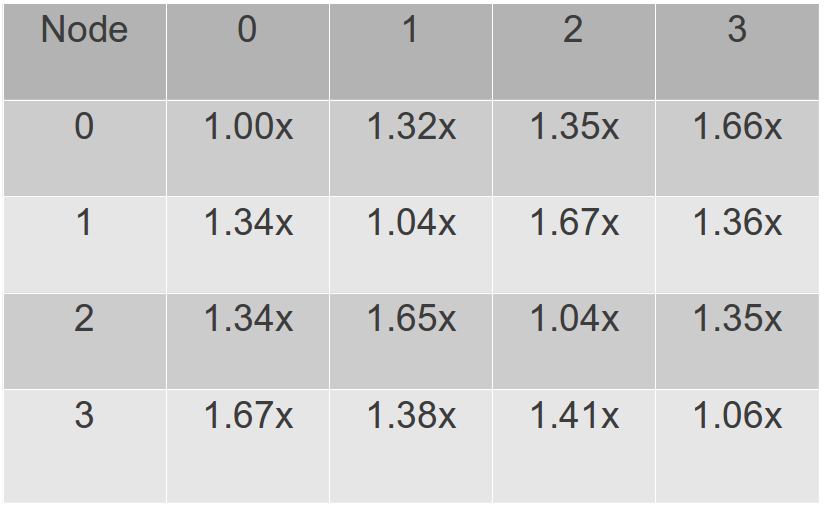
\includegraphics[scale=0.35]{numaMatrix.png}
    \caption{This shows the slowdown between each node. }
    \label{fig:numaMatrix}
\end{figure}

\textbf{NUMA APIs - }
In this section we will look into some of the libraries exposed for programmers to control data allocation and thread allocation for NUMA machines.
Cache related and topology related information about the NUMA hardware can be found at:
 
\texttt{/sys/devices/system/cpu/cpu*/cache } \\
\\
\texttt{ /sys/devices/system/cpu/cpu*/topology }

\textit{numactl} is a library which we have used for this work.
It has various APIs which can control the cores and nodes to which the process and data can be bound.
We have used \textit{pin_to_core()} function to pin a specific thread on a given core.
Similarly \textit{numa_alloc_onnode()} allows the programmer to allocate data on a specific node.
\textit{numactl} also has various command-line arguments like \textit{cpubind} and \textit{membind} to bind processes and data to specific nodes.
And the \textit{hardware} flag provides info about the underlying NUMA hardware.
